\documentclass{beamer}

\usepackage[utf8]{inputenc}
\usepackage[english]{babel}
\usepackage[T1]{fontenc}
\usepackage{listings}
\usepackage{xcolor}

% font
\usefonttheme{serif}

% theme
\usetheme{default}
\setbeamertemplate{navigation symbols}{}

% colors
\usecolortheme{beaver}
\definecolor{myred}{HTML}{cc0000}
\setbeamercolor{block body}{bg=black!5}
\setbeamercolor{block title}{bg=black!10,fg=myred}

% progress
\AtBeginSection[]
{
\begin{frame}
  \frametitle{Outline}
  \tableofcontents[currentsection]
\end{frame}
}
% \AtBeginSubsection[]
% {
% \begin{frame}
%   \frametitle{Outline}
%   \tableofcontents[currentsubsection]
% \end{frame}
% }
% \setbeamertemplate{footline}[frame number]

% default graphics path
\graphicspath{{inc/graphics/}}

% listings config
\lstdefinestyle{colored}{ %
  basicstyle=\ttfamily,
  backgroundcolor=\color{white},
  commentstyle=\color{green}\itshape,
  keywordstyle=\color{blue}\bfseries\itshape,
  stringstyle=\color{red},
}
\lstset{
  aboveskip=1em,
  breaklines=true,
  abovecaptionskip=-6pt,
  captionpos=b,
  escapeinside={\%*}{*)},
  frame=single,
  numbers=left,
  numbersep=15pt,
  numberstyle=\tiny,
  style=colored
}

% title page
\title{Python Package for World Wide Statistics Visualization}
\subtitle{}
\titlegraphic{
\includegraphics[height=2.5cm]{./inc/graphics/fds.png}}
\author{\footnotesize{Sophie Manuel, Ravahere Paint-Koui, Seydou Sane, Anas Zakroum}}
\date{\today}
\institute{Université de Montpellier}

%%%%%%%
%%%%%%%
%%%%%%%

\begin{document}

\begin{frame}[plain]
  \titlepage
\end{frame}

\small
\begin{frame}[plain]
  \frametitle{Outline}
  \tableofcontents
\end{frame}
\normalsize

\section{Introduction}
\begin{frame}
  \frametitle{Introduction}
  \framesubtitle{Motivation of this work}
% there exist many python packages for generating plots such as matplotlib,
% plotly, seaborn, etc.. However, the end user needs to read a long long
% documentation to get used to it.

% what about aggregating all of these packages into one simple "easy to use" 
% package, a task-oriented package (i.e. to perform a specific task).

% we choose as a proof-of-concept the task consisting of visualizing world wide
% statistics.
\end{frame}

\begin{frame}[fragile,shrink=30]
  \frametitle{Introduction}
  \framesubtitle{Quick Example}
 
  \begin{lstlisting}[language=Python,numbers=left]
  from wwstatviz import Visualizer

  v = Visualizer('/path/to/data.csv')
  fig = v.choropleth(title = '...', 
                     feature = 'GDP',
                     countries = ['FRA', 'USA', 'AFG', ...])
  fig.save('/path/to/output_file.png')
  \end{lstlisting}

  \begin{lstlisting}[language=Python,numbers=left]
  fig = v.heatmap(title = '...',
                  features = 'all',
                  countries = ['ALG', 'GER', 'SEN', ...])
  fig.show() # for inline display (in browsers for example)
  \end{lstlisting}
\end{frame}


\section{Package wwstatviz - API}
\begin{frame}
  \frametitle{API}
% it's a python package presenting an API for simple generation of
% visualizatons

Available plots in the current state are:
\begin{itemize}
  \item choropleth: ...
  \item heatmap: ...
  \item line plot: ... for time series visualization
  \item histogram: ...
\end{itemize}
% It's in active development, we will extend it to more widgets in the future
\end{frame}

\begin{frame}[fragile,shrink=30]
  \frametitle{Package structure}
\begin{verbatim}
wwstatviz
|-- __init__.py
|-- generators/
|   |-- __init__.py
|   |-- choropleth.py
|   |-- generator.py
|   |-- heatmap.py
|   `-- line.py
|-- io/
|   |-- __init__.py
|   |-- csvreader.py
|   |-- jsonreader.py
|   |-- iso.py
|   |-- reader.py
|   `-- writer.py
|-- figure.py
`-- visualizer.py
\end{verbatim}
\end{frame}

\begin{frame}[fragile,shrink=10]
  \frametitle{The Visualizer Class}
  \framesubtitle{Input Data}
  
  The constructor of the class take as input a data file \\
  (in the CSV format):
  \begin{itemize}
    \item The first line must contain the header
    \item Each row must start with a country code (ISO-3166 2-digit or 3-digit)
    \item The columns (i.e. the features) represent the data
  \end{itemize}
  
  \vspace{5mm}
  
  Example:
  \begin{verbatim}
    ,f1,f2,f3
    AFG,0,1,2
    BEL,5,4,3
    FRA,6,7,8
    SEN,12,13,14
    USA,3,33,8
  \end{verbatim}

\end{frame}

\begin{frame}
  \frametitle{The Visualizer Class}
  \framesubtitle{Main functions}

  \begin{itemize}
    \item This Visualizer class is the main interface of the API.
    \item The constructor (\_\_ini\_\_(self, data\_path)) takes as input 
      the path to the data file
    \item It contains functions for generating graphics (choropleth, histogram, etc.)
    \item These function are simple calls to the Generators
    \item Each function returns a Figure object (for later use)
  \end{itemize}

\end{frame}

\begin{frame}[fragile,shrink=30]
  \frametitle{Generators}

  About Generators:
  \begin{itemize}
    \item Generators are responsible for producing plots.
    \item Each generator should inherit from the base class 
      ``Generator'' and must implement a ``generate()'' method
    \item The generator contructor takes as argument the different options 
      to be used for generating the plots 
      (e.g. whether or not to draw a legend, the countries to use, etc.)
  \end{itemize}

  \vspace{5mm}

  Example:
  \begin{lstlisting}[language=Python]
  class XYZGenerator(Generator): # class inheritance
      
      def __init__(self, ...): # this is the contructor
          ...

      # generate method must be implemented 
      # and must return a figure
      def generate(self): 
          ...
          return figure
  \end{lstlisting}
\end{frame}

\begin{frame}
  \frametitle{Input/Output module}
  About the ``io'' module:
  \begin{itemize}
    \item The io module is Responsible for:
      \begin{itemize}
        \item reading data files from disk for different 
          formats (csv, json, etc.) % json is not implemented yet
        \item writing generatred figures to disk
      \end{itemize}
    \item It contains the base classes Reader and Writer
    \item For each data format, a reader submodule must be implemented
    \item Each reader submodule (e.g. csvreader) should implement a class that:
      \begin{itemize}
        \item inherits from the base class ``Reader''
        \item implements a ``read()'' method
      \end{itemize}
  \end{itemize}
\end{frame}


\section{Continuous Integration}
\begin{frame}
    \frametitle{Continuous Integration}
    %practice of 
    \begin{itemize}
        \item Automating integration of code changes
        \item From multiple collaborators
        \item Into a single project
        \item Avoid merge problems
    \end{itemize}
    
\end{frame}

\begin{frame}
    \frametitle{Continuous Integration}
    \framesubtitle{wwstatviz}
    
    \begin{itemize}
        \item Check requirements and install dependencies
        \item Test with pytest
        \item Check for PEP8
    \end{itemize}
\end{frame}

\section{Unit Tests}
\begin{frame}[fragile,shrink=30]
  \frametitle{Unit Testing Using pytest}
  
  % what is unit testing

  The tests are performed through assertions:
  \begin{itemize}
    \item Whether or not the figure is generated
    \item The instance of the generated plot (a matplotlib figure, a plotly figure, etc.) 
    \item The writing of the generated figure in disk
  \end{itemize}

  \vspace{5mm}

  Example:
  \begin{lstlisting}[language=Python]
    v = Visualizer('/workspace/data/test_cc_3d.csv')
    fig = v.heatmap(title = 'This is a test heatmap',
                    xlabel = 'Countries', ylabel = 'Countries')
    assert fig.figure is not None
    assert isinstance(fig.figure, matplotlib.figure.Figure)
    fig.save('test_heatmap.png')
    assert Path('test_heatmap.png').is_file()
  \end{lstlisting}

  \begin{figure}[h]
    \centering
    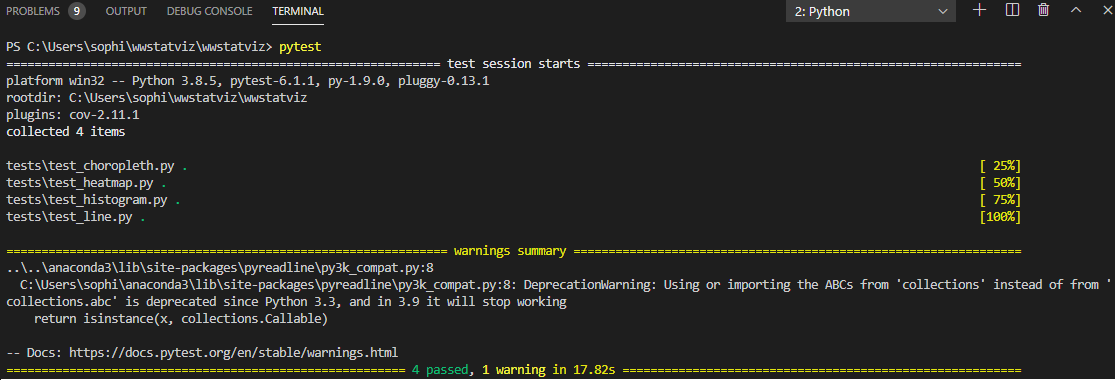
\includegraphics[scale=0.3]{tests.png}
    \caption{Unit Test Exection}
    \label{fig:tests}
  \end{figure}
  

\end{frame}


\section{Demo}
\begin{frame}[fragile,shrink=30]
   \frametitle{Choropleth}
   \begin{lstlisting}[language=Python]
    v = Visualizer('path/to/file.csv')
    fig = v.choropleth(title = '...',
                  features = 'all',
                  countries = 'all')
    fig.show() # for inline display (in browsers for example)
    \end{lstlisting}
    \begin{center}
        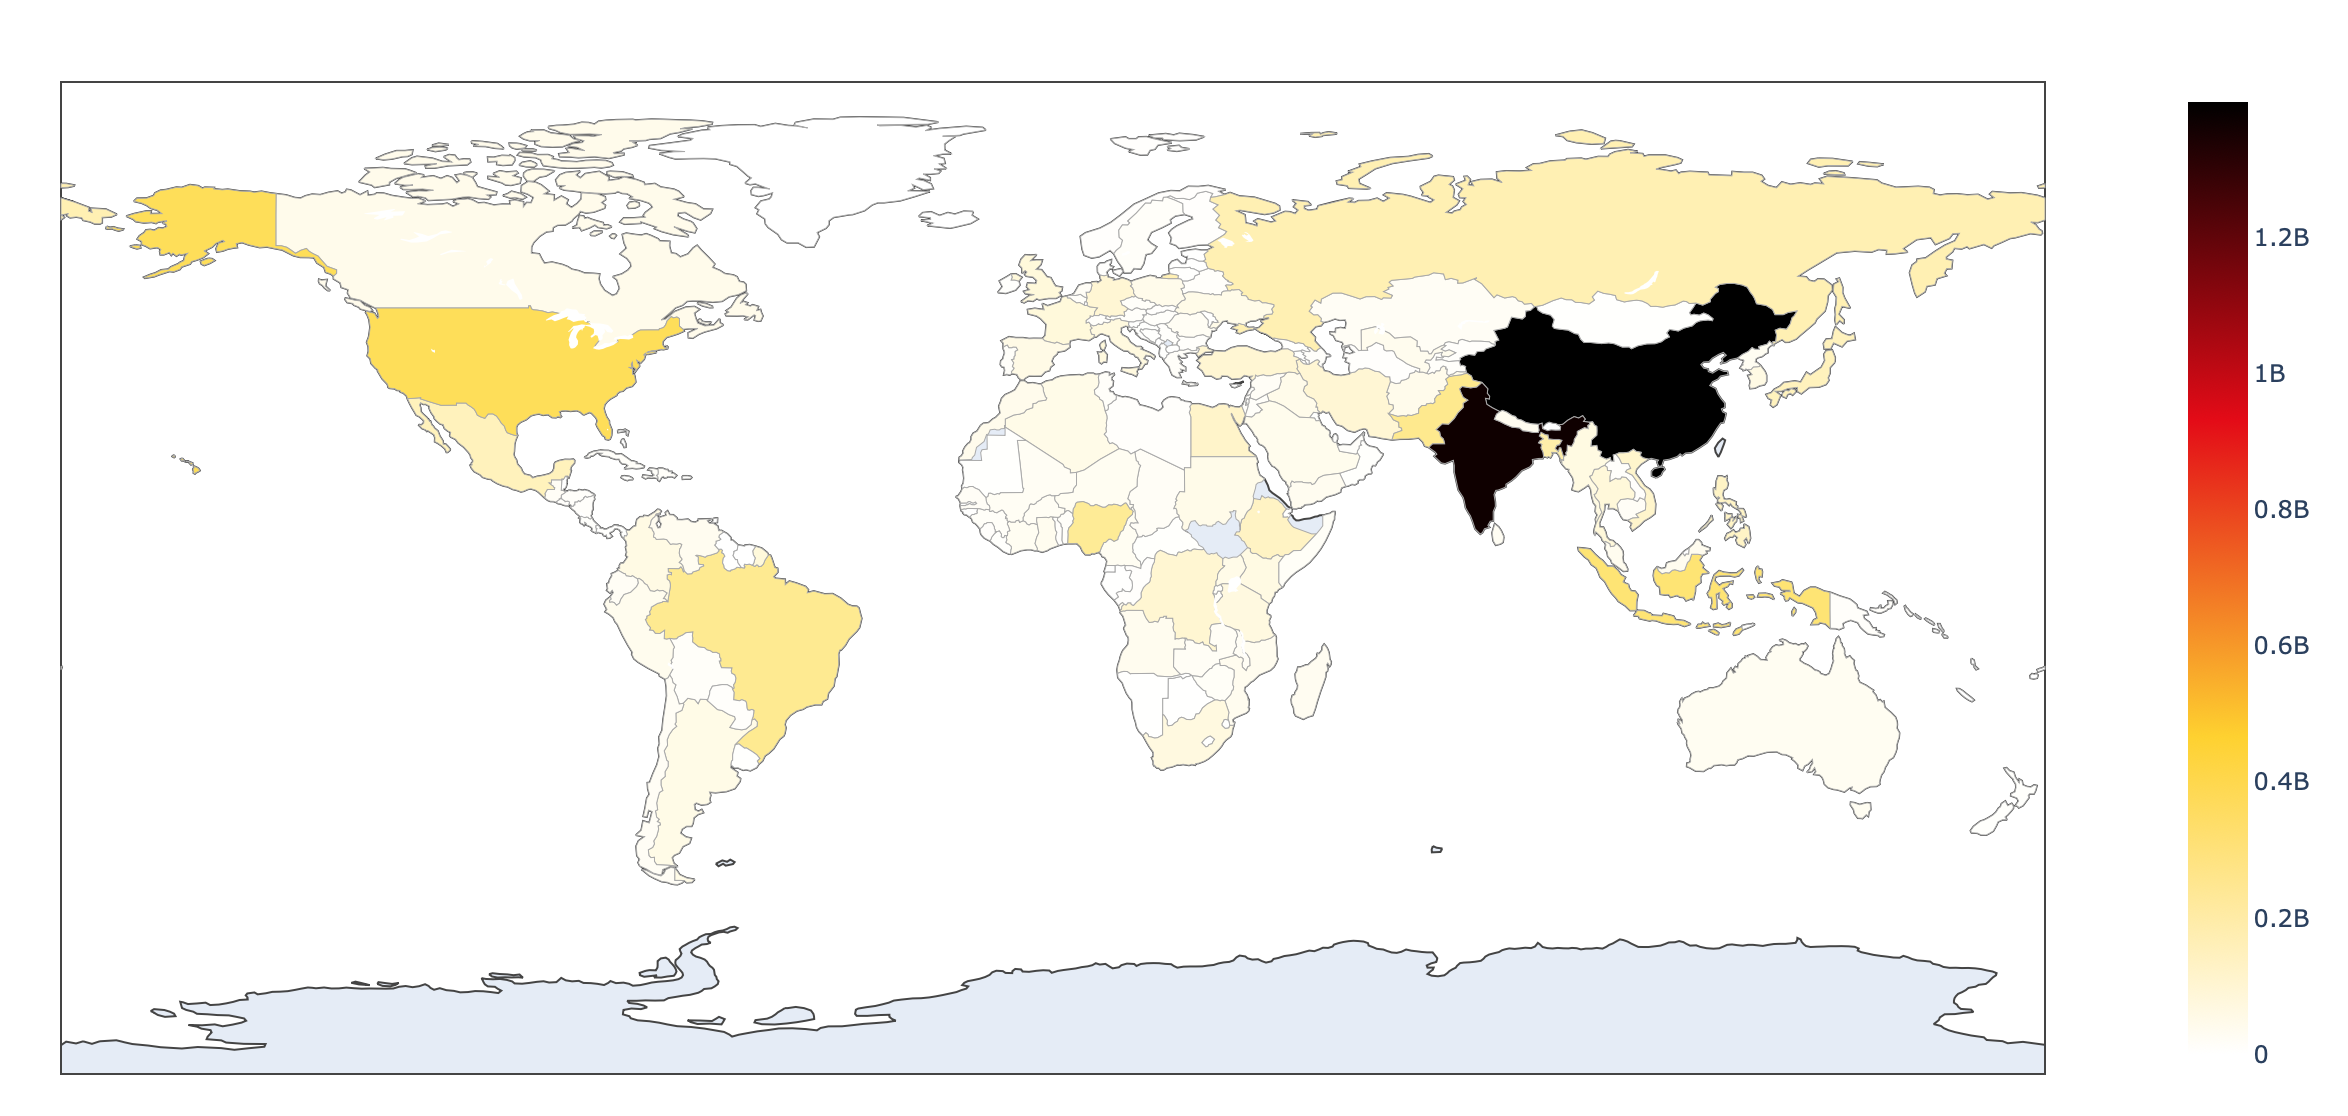
\includegraphics[scale=0.4]{beamer/inc/graphics/choropleth.png} 
    \end{center}
\end{frame}

\begin{frame}[fragile,shrink=30]
  \frametitle{Heatmap}
  \begin{lstlisting}[language=Python]
  v = Visualizer('path/to/file.csv')
  fig = v.heatmap(countries='all', features='all',
                    method='pearson', mask=True,
                    title='This is a test heatmap', xlabel='Countries', ylabel='Countries')
  fig.show() #for inline display (in browsers for example)
  \end{lstlisting}
  \begin{center}
    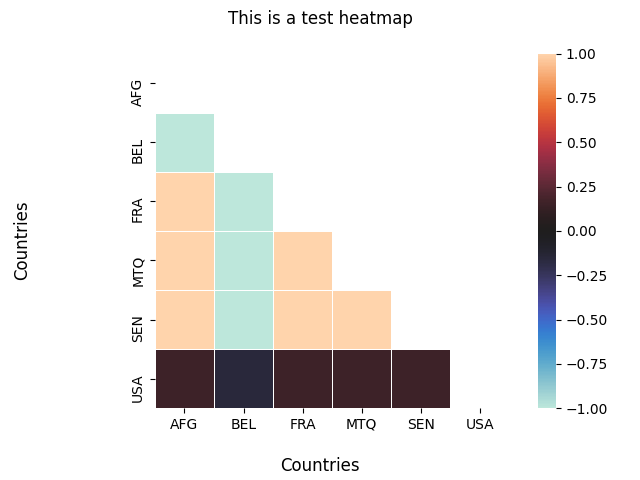
\includegraphics[scale=0.6]{beamer/inc/graphics/heatmap.png}
    \end{center}
\end{frame}

\begin{frame}[fragile,shrink=30]
  \frametitle{Time Series Plot}
  \begin{lstlisting}[language=Python]
    v = Visualizer('path/to/file.csv')
    fig = v.line(countries='all', features='all',
              title='This is a test of line plot', xlabel='Label of x axis', ylabel='Label of y axis', 
              legend=False)
    fig.show() # for inline display (in browsers for example)
      \end{lstlisting}
    \begin{center}
    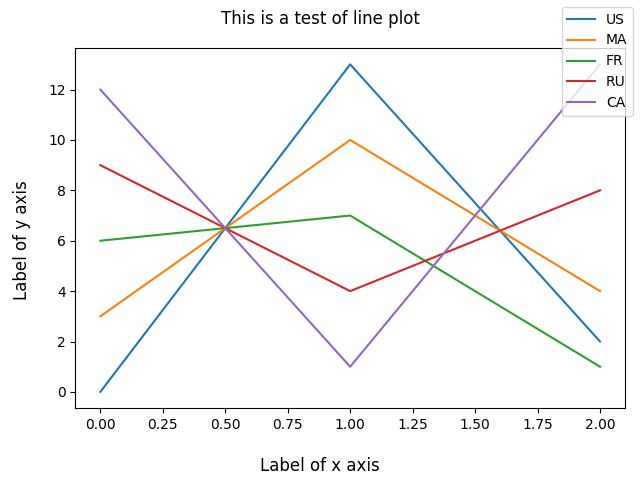
\includegraphics[scale=0.6]{beamer/inc/graphics/line.png}
    \end{center}
\end{frame}

\begin{frame}[fragile,shrink=30]
  \frametitle{Histogram}
    \begin{lstlisting}[language=Python]
    v = Visualizer('path/to/file.csv')
    fig = v.histogram(countries='all', features='all',
                    title='This is a test histogram', xlabel='Label of x axis', ylabel='Label of y axis', 
                    legend=False)
    fig.show() # for inline display (in browsers for example)
    \end{lstlisting}
    \begin{center}
    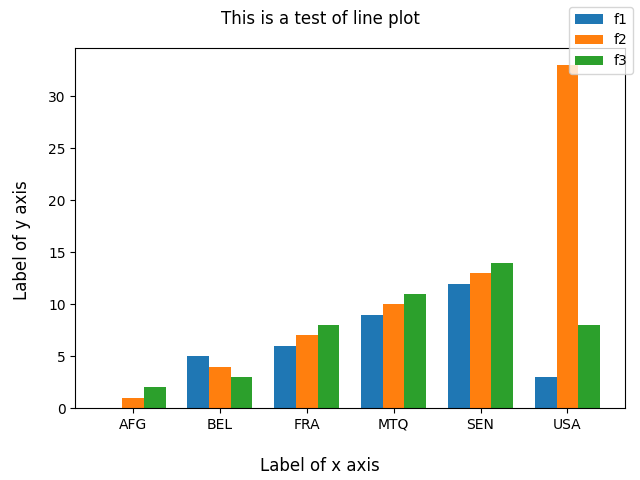
\includegraphics[scale=0.6]{beamer/inc/graphics/histogram.png}
    \end{center}
\end{frame}

\section{Package wwstatviz-webapp - User Interface}
\begin{frame}
  \frametitle{A Web Application}
  % facilitate the usage for non-developer end-users
  % what it does, see readme
  % it is intuitive
  % As a backend, it uses a minimalistic and efficient python web framework: flask
  % it's in active development
\end{frame}

\begin{frame}
  \frametitle{About Flask}
  % search the internet and explain the concept here
  % put a simple example of code (the one they provide in the quickstart of the
  % doc)

  \begin{itemize}
    \item micro web framework for Python;
    \item handy to launch small applications or web page
  \end{itemize}

The following code aims at displaying "Hello World!" on a web page: 

  \begin{lstlisting}[language=Python,numbers=left]
    from flask import Flask
    app = Flask(__name__)

    @app.route("/")
    def hello():
        return "Hello World"


    if __name__ == "__main__":
        app.run(debug=False)
  \end{lstlisting}

\end{frame}


\section{Conclusion}
\begin{frame}[fragile]{Conclusion}

\centering
\begin{block}{What we learnt}
    \begin{itemize}
        \item Learn more about geospatial visualization techniques;
        \item Create one package from several Python packages.
    \end{itemize}
\end{block}

\begin{block}{What can be improved}
    \begin{itemize}
            \item A web application;
            \item More custom options for the figures we are able to create.
        \end{itemize}
\end{block}

\end{frame}

\AtEndDocument{
    \begin{frame}
                \centering
                \Large
                \newline
                Thank you for your attention!
                \newline
                \newline
                \newline
                \newline
                \newline
                \newline
                \newline
                \newline
                \newline
                \newline
                \newline
                \newline
                \newline
                \tiny
                \begin{flushleft}
                You can get more information about wwstatviz on:
                \newline
                \newline
                \href{https://github.com/SophieManuel/wwstatviz}{\beamergotobutton{wwstatviz github}}    
                \end{flushleft}
                
    \end{frame}
                }

\end{document}
